\chapter{基于语义扩展和文本质量的实时个性化搜索}
\label{2chap:main}
随着社交网络中信息爆炸式的增长,用户越来越难以从海量的信息中获取到自身所需的信息,用户所需的信息往往淹没在其中,这种现象可称之为\textbf{信息洪流}(\textit{information flood})现象。在社交网络、电子商务网站、即时通信等应用中,信息产生的速率以及数量都是过去无法比拟的,如在推特(Twitter)、脸书(Facebook)、新浪微博等社交媒体中,每天都会产生海量的文本信息。根据用户输入的查询,在海量的信息流中实时地检索出高质量的、相关的信息是一个极具挑战性的问题。社交网络中的信息流实时个性化搜索相对于传统的信息检索提出了以下挑战:(1)社交网络中充斥着各种各样话题的信息,而且信息大多数都是以短文本表示,相对于传统的新闻等长文本信息,难以进行语义理解;(2)社交网络中的信息质量参差不齐,难以从中遴选出高质量的信息;(3)社交网络中的信息产生速率快,如何能够实时地检索出用户所需要的信息,将其推送给用户也是一大难点。因此,由于社交网络中数据的信息海量性、主题多样性、数据稀疏性以及社交互动性等特性,传统的个性化检索方法不足以解决社交网络中的信息实时个性化搜索问题。本章针对以上的问题,提出了一个面向推特信息流的实时个性化搜索框架来实现用户的信息实时推荐。本章针对社交网络中信息的特性,提出了一种基于语义扩展和文本质量的实时个性化搜索算法,并在TREC 2015 Microblog Track\upcite{lin2015overview} 测评中验证了算法的性能。首先,我们构造了一个逻辑规则过滤器来选择核心关键词,提高检索的准确率。其次,我们对文本质量进行建模,利用的标注的数据进行训练,以此来对文本的质量的进行打分。训练好的文本质量模型提高了检索的排序性能。然后,我们使用外部语料库来实现语义扩展,例如搜索引擎,知识库等。语义扩展能够使得我们更好地理解用户的偏好和兴趣。最后,我们采用了一个动态的推送策略来自动地推送高质量且相关的信息给特定的用户,这能够避免信息过载。本章中的算法结合了社交网络文本的语义特征和社交属性,针对不同的用户搜索,做了综合性地排序。我们使用TREC 2015 Microblog Track中的真实数据流进行了实验,实验结果显示了本章提出的算法在不同测评指标下,与其他算法相比的优越性。

本章的内容组织如下:第\ref{2sec:motivation} 节介绍了研究动机,讨论了在社交网络环境下进行实时个性化搜索的必要性。第\ref{2sec:definition}节介绍了相关定义,对本章中涉及的相关概念和知识进行了符号化的定义。第\ref{2sec:method} 节介绍了方法描述,详细地阐述了本章提出的系统框架和算法。第\ref{2sec:experiment}节进行了实验分析,验证了本章提出的方法,并且分析了实验结果。最后,第\ref{2sec:conclusion}对本章的内容进行了总结。

\section{研究动机}
\label{2sec:motivation}
随着大数据时代的到来,诸如推特(Twitter)、脸书(Facebook)、新浪微博等的社交网络平台逐渐取代传统的媒体平台,成为新时代的实时信息交互平台。以推特平外为例,据统计,每天平均约有58,000,000条推文(tweet)发布,每天平均处理约2,100,000,000次搜索查询,每月约有115,000,000个活跃的用户\footnote{\url{http://www.statisticbrain.com/twitter-statistics/}}。 在大数据时代,人人都可以是信息的生产者、传播者和接收者,这在一定程度上加速了信息的传播速率。然而,如此庞大的数据量使得用户在社交网络平台中搜索查询时面临了信息过载的问题,用户很难检索到自己需要的信息,亦或用户所需的信息淹没在了众多的信息之中。尤其是社交网络平台中的信息内容囊括了众多领域,其中的话题种类繁多,这使得用户难以搜索到相关性强而且高质量的文本信息。在社交网络平台中,传统的信息检索方法变得耗时长而且信息检索方式难以适用。因此,在大数据时代,为了满足用户实时获取相关信息的需求,需要一种面向社交网络的新的信息检索方法。

在传统的信息检索流程中,往往是用户根据自己所需,输入关键字进行查询,系统根据用户的查询,搜索到相关的结果,并进行排序,返回给用户。而在社交网络平台中,信息产生速率快,信息以数据流的形式给出,同时用户希望系统能够自动地推送相关的信息,而不是用户通过查询来获取信息。因此,在社交网络中的信息实时个性化搜索的流程与传统的信息检索流程不尽相同。在社交网络中,信息的实时个性化搜索流程一般是用户将查询搜索以关键词的形式给出,然后系统根据用户的查询在信息流中实时地处理文本信息,将相关的信息自动地推送给用户。

由美国国家标准与技术研究院(NIST)主办的文本检索会议(TREC)是由多个测评项目组成的一个致力于解决新时代信息检索问题的测评大会,涉及智能问答、医疗诊断、实体识别、信息推荐等领域。TREC自2011年起设立了微博实时推荐(Microblog Track)\upcite{ounis2011overview,soboroff2012overview,lin2013overview,lin2014overview,lin2015overview} 这一个子任务,目标是解决在社交网络中信息的实时个性化搜索问题。从设立后,TREC Microblog Track便吸引了全世界的参赛者参加,与智能实时问答(TREC LiveQA Track)成为了TREC中最火热的两个子任务。Microblog Track 的任务是针对不同用户,智能地分析用户的兴趣爱好,自动地、实时地为用户推送相关的、高质量的信息,涉及到众多科学领域,包括机器学习、自然语言处理、信息检索、人工智能等。如图\ref{fig:twitter_search}所示,在社交网络平台中,用户是信息的生产者,用户将源源不断地发布信息,其中包括有趣的信息和一些无用的信息。同时,用户又是信息的接收者,用户通过定制自身感兴趣的话题和内容,系统智能地分析其兴趣爱好,针对不同的用户,在推特信息流中自动地、实时地为用户推荐相关的、高质量的信息。例如将饮食信息推荐给美食家、将财经信息推送给金融家、将商旅信息推送给旅行者等,同时将一些低质量无意义或者无人关注的信息丢弃。

\begin{figure}[!htbp] % use float package if you want it here
  \centering
  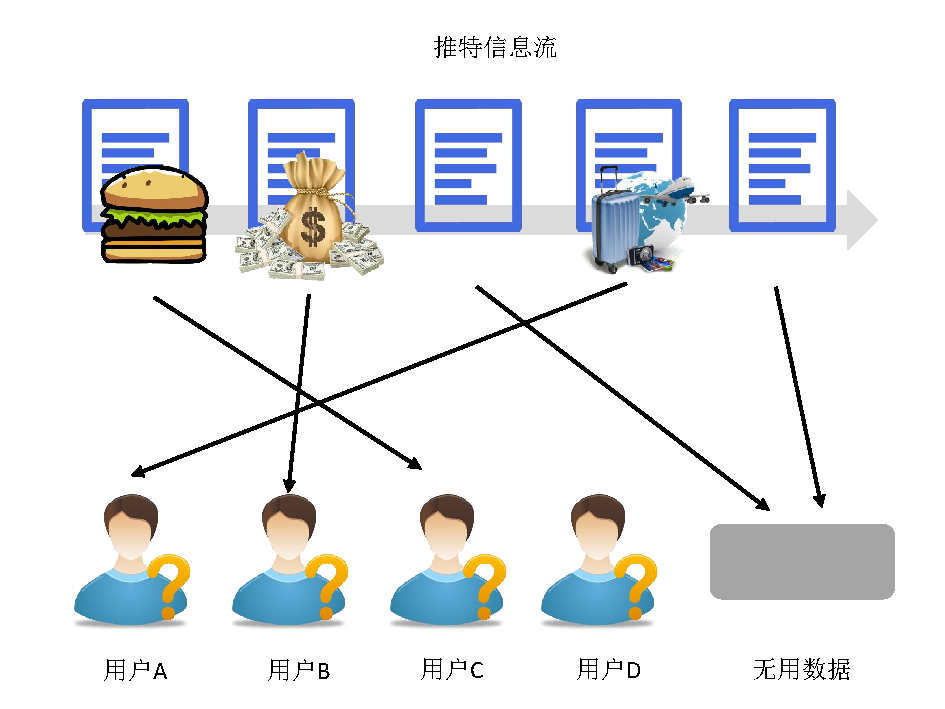
\includegraphics[width=0.8\textwidth]{twitter_search}
  \caption{社交网络平台中信息的实时个性化搜索示意图}
  \label{fig:twitter_search}
\end{figure}

为了解决针对不同用户,为其实时地搜索出相关性强、高质量的信息,许多已有的个性化推荐\upcite{Xie2015Personalized,sontag2012probabilistic,wang2013personalized,tang2015personalized} 以及协同搜索\upcite{liang2014Collaborative,vosecky2014collaborative,xue2009user,yang2014survey} 的工作对这个问题进行了一定的研究。但是很少有面向社交网络个性化搜索的研究,特别是对于实时搜索推荐技术的研究。目前已有的机器学习、自然语言处理、信息检索、人工智能等研究对于社交网络中的实时个性化搜索问题提供了许多帮助。文本分类以及排序的研究\upcite{canuto2015efficient,severyn2015learning,ren2014hierarchical,paik2013novel} 能够为了社交网络中的信息检索提供支持。同时,查询分析以及优化技术\upcite{gao2013query,Letelier2012Static,si2014users} 能够使得信息检索有着显著的提升。

然而,社交网络的环境与传统的新闻、论坛等Web环境有着较大的区别。因此,为了满足社交网络中用户获取信息的需求,这将需要建立新的模型、研究新的方法来解决这一问题。在社交网络中,实现信息的个性化实时推荐面临的主要挑战可以总结如下:
\begin{itemize}
  \item \textbf{信息海量性},在社交网络中,信息产生的速率快,网络中的每一个用户同时扮演着信息生产者、信息传播者和信息接收者的角色。如此高容量的信息流需要一个新的模型来适应持续不断变化的语义特征。
  \item \textbf{主题多样性},社交网络中的信息内容包罗万象,覆盖了许许多多的领域和话题。如果主题模型不能区分众多的话题,这将导致噪声的引入以及不准确的话题模型以及用户模型。
  \item \textbf{数据稀疏性},在社交网络中,信息在不同的主题上的分布是不均匀的,在某些主题上信息量大,而在某些主题上信息是稀疏的。有效的主题模型需要解决数据稀疏性所带来了的影响。
  \item \textbf{社交互动性},社交网络中的用户之间有着丰富的互动信息,与传统的文本信息不同,社交网络中的信息包含了许多有价值的结构化的社交属性。适当地利用这些社交属性能够提高搜索的性能,但是这需要对这些社交属性进行相关性的选择。
\end{itemize}

为了解决上述面临的挑战,本章提出了一种基于语义扩展和文本质量的实时个性化搜索框架,该框架综合考虑了用户的偏好、语义特征和社交属性。首先,本章基于语义扩展提出了一种布尔逻辑关键词过滤(Boolean Logic Keyword Filter)的用户模型。该模型依靠外部搜索引擎提供的知识进行建立,建立的用户模型充分利用了查询扩展以及检索结果的重排序来提高推荐结果的相关性。最终的实验评估证明该模型显著地提高了检索的召回率。此外,本章还基于逻辑回归提出了一种文本质量模型,该模型利用推文的社交属性来评估其文本的质量。该模型能够对推文的文本内容,是否受到大众的认可等进行评估,因此它能帮助系统返回高质量的推文。最终的实验评估证明该模型显著地提高了检索结果的排序性能。

\section{相关定义}
\label{2sec:definition}
本节首先将对社交网络中的实时个性化搜索的任务进行定义,并将其形式化,然后对TREC 2015 Microblog Track的具体任务进行描述。

社交网络中的实时个性化搜索任务可以描述如下。在社交网络中平台中,令信息流表示为\textbf{T},信息流在社交网络中随着时间不断地产生,信息流\textbf{T}中包含许多种类的话题。令\textbf{P}表示用户集合,每一个用户$p_i \in \textbf{P}$表示着用户感兴趣的一个话题,用户的兴趣爱好可以通过文本等形式来表示。则社交网络中的实时个性化搜索任务可以定义如下,
\begin{mydef}[实时个性化搜索]\label{def:realPrnzdSearch}
在社交网络中,给定信息流\textbf{T}以及用户集合\textbf{P},实时个性化搜索的目的是针对不同的用户兴趣爱好$p_i \in \textbf{P}$,自动地实时地为其推荐高质量的、相关的信息。
\end{mydef}

根据定义\ref{def:realPrnzdSearch}可知,社交网络中的实时个性化搜索需要解决的几个核心关键问题如下。首先是如何表示信息流与用户,其次是如何实现实时推荐,以及如何保证信息的高质量和高相关性。社交网络中的实时个性化搜索任务可以通过图来表示。

TREC 2015 Microblog Track的任务目标是\textbf{实时信息流过滤},实质上也是实时个性化搜索的一种形式。在Microblog Track中,实时信息流过滤的任务目标是根据不同用户的兴趣模型来监测社交媒体中的信息流。值得注意的是,上述的兴趣模型的概念是不同于传统的临时查询。该场景中,交互流程不是用户输入一次查询,然后系统返回结果给用户。该场景不存在实际的查询,取而代之的是系统根据用户的兴趣模型主动地推送\textbf{有趣的}信息给用户。

上述什么样的信息是有趣的可以考虑如下两个实际的任务模型来帮助更好地理解。
\begin{itemize}
  \item \textbf{场景A:即时性信息推送},在场景A中,用户是定位在使用移动设备的场景,用户可以即时地查看消息。系统基于用户的兴趣模型来判别消息之于用户是否是有趣的,被系统判别为有趣的信息将实时地推送到用户的移动设备(例如手机、平板等)。场景A中的任务目的是上述的推送需要在消息产生的相对较短的时间内完成,该场景中的信息假设是相对较短的。
  \item \textbf{场景B:周期性邮件摘要},在场景B中,用户是定位在使用固定设备的场景,用户周期性的查看消息。与场景A相同,统基于用户的兴趣模型来判别消息之于用户是否是有趣的。但是被系统判别为有趣的信息将被聚集成一个邮件摘要,并且周期性的推送给用户。该场景中的每一个单一信息假设是相对较短的,聚集成的邮件摘要可能很长,我们可以认为这是\textbf{个性化头条新闻}。
\end{itemize}

两个场景都假设推送给用户的消息相对较短,是短消息。因此,推送的消息是否有趣可以根据用户阅读消息的长度或者条数来进行衡量。

在实时信息流过滤任务中,信息即为推文。在测评阶段,进行测评的系统将监测推特的实时样本信息流并根据用户的兴趣模型(相当于特定的话题)来识别有趣的信息。为了描述的简洁性,我们将上述过程称之为\textbf{兴趣用户的追踪}。

\section{方法描述}
\label{2sec:method}
在本节中,我们设计了一个面向社交网络的实时信息流推荐的系统框架。首先,与传统的信息检索系统相似,信息以及用户的语义特征被提取出来,数据的预处理用于过滤掉此阶段中无用的信息。其次,为了计算信息与用户之间的相似度(即相关性),基于外部语料库训练得到的词向量模型来表述提取的特征。除此之外,系统将文本的质量也考虑在内。高质量的文本往往包含高质量的信息,本节提出了一个基于逻辑回归模型的文本质量评估算法来对文本的质量进行衡量。然后,基于得出的相关性与质量,系统针对不同的用户对信息进行评估。一条相关的、有意思的信息将被归类到最相关的类别中,即归类到最相关的用户。最后,为了避免信息洪流、保持消息推送的实时性,本节提出了一个动态的推送策略。因此,用户将实时地收到相关性强、质量高的信息,并且能够避免淹没在信息中。

\section{实验分析}
\label{2sec:experiment}

\section{本章小结}
\label{2sec:conclusion}


